\begin{frame}[hasprev=false,hasnext=false]
\label{example:functional-testing}
\frametitle{Functional testing example}

Consider the function $x^y$, where $x$ is an integer and $y$ is a non-negative
integer. The input domain is: for every tuple (x,y), with $y >= 0$. The input
domain can be partitioned as follows:

\begin{figure}
    \centering
    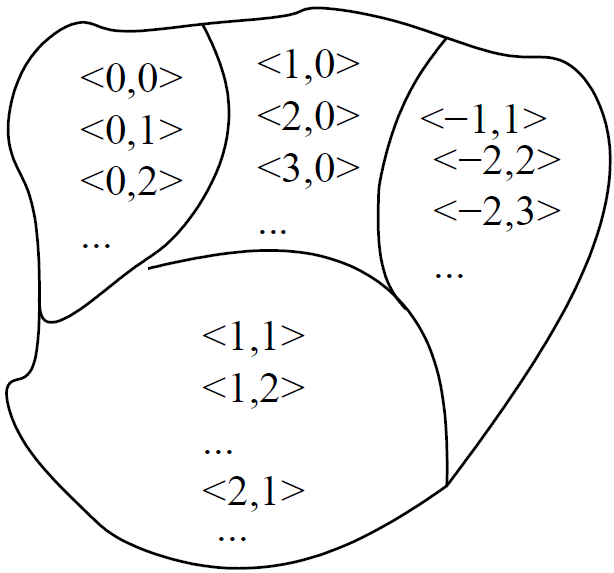
\includegraphics[width=4cm]{aux/examples/functional-testing/functional-testing}
\end{figure}
\end{frame}

